% !TEX encoding = UTF-8
\documentclass[a4paper,12pt,titlepage=true, ngerman]{scrartcl}
%\usepackage{ngerman}, 
%\usepackage[ngerman]{babel}

\usepackage[utf8]{inputenc}
\usepackage[ngerman]{babel}
\usepackage[babel]{csquotes}

\usepackage[backend=biber, style=authoryear-comp, maxbibnames=3,
 isbn=false, doi=false, eprint=false, dashed=false]{biblatex}
 
\ExecuteBibliographyOptions{maxcitenames=2}

\bibliography{literature.bib}
\usepackage{hyperref}
%\hypersetup{
%colorlinks=true, linktocpage=false, pdfborder={0 0 0}, pdfstartview=FitV, 
%urlcolor=Black, linkcolor=Black, citecolor=Black, %pdfstartpage=3, 
%}
\usepackage{graphicx}

\usepackage{scrhack}
\KOMAoptions{BCOR=8mm}
%\KOMAoptions{toc=flat}
% \KOMAoptions{toc=graduated, toc=bibliography}

% \renewcommand*\sectfont{\rmfamily\mdseries\scshape}
\setkomafont{section}{\rmfamily\bfseries\LARGE}
% \setkomafont{sectionentry}{\rmfamily\bfseries\scshape\Large}
\setkomafont{subsection}{\rmfamily\bfseries\Large}
\setkomafont{subsubsection}{\rmfamily\bfseries\large}
%\setkomafont{chapter}{\rmfamily\bfseries\scshape\huge}
%  \setkomafont{partentry}{\rmfamily\bfseries\scshape}
% \setkomafont{chapterentry}{\rmfamily\bfseries\scshape}
\setkomafont{partentry}{\rmfamily\bfseries\scshape}
\setkomafont{part}{\rmfamily\bfseries\scshape\huge}
\setkomafont{partnumber}{\rmfamily\bfseries\scshape\huge}
\setkomafont{partentrypagenumber}{\rmfamily\bfseries\scshape}

\setkomafont{descriptionlabel}{\bfseries}

%  scrhack to fuck float error message

%%%%  for page head and foot %%%%%%%
\usepackage[automark]{scrpage2}
\pagestyle{scrheadings}
\KOMAoptions{headsepline=true}
\setheadsepline{.4pt}
\setkomafont{pageheadfoot}{\normalfont\normalcolor\upshape} 

\setcounter{tocdepth}{3}
\setcounter{secnumdepth}{4}

\usepackage[T1]{fontenc} % to make Sa\"ibi searchable
\usepackage[protrusion=true,expansion=true]{microtype}
% \usepackage{microtype}
% \usepackage{setspace}\setstretch{1.2}



% \usepackage{lmodern} 


%  \usepackage{palatino}\linespread{1.05}
 \usepackage{mathpazo}\linespread{1.05}  
\usepackage[scaled=.95]{helvet}
   \usepackage{courier}
   \usepackage[scaled]{berasans}
 
% \usepackage[bitstream-charter]{mathdesign}  %%%%%%%%%%%%%%%%%%%%%  FINAL VERSION %%%%%%%%%%%%%%%%%%%%%%%%%%%%%%%

%\usepackage[style=authoryear,
% 	maxnames=1,
%  	maxbibnames=99,                  %%%%%%%%     TODO  activate
% uniquename=init
%]{biblatex}

\usepackage{calc}
\usepackage{ifthen}

\usepackage{tikz}
\usetikzlibrary{shapes,arrows}

\tikzstyle{task} = [diamond, draw, fill=green!20, 
    text width=4.5em, text badly centered, node distance=2cm, inner sep=0pt]
\tikzstyle{comp} = [rectangle, draw, fill=blue!20, 
    text width=5em, text centered, rounded corners, minimum height=4em, node distance=2cm]
\tikzstyle{line} = [draw, -latex']
\tikzstyle{line2} = [draw, double, -latex']
\tikzstyle{human} = [draw, ellipse,fill=red!20, text width=5em, text centered, node distance=2cm,
    minimum height=3em]
\tikzstyle{decision} = [diamond, draw, fill=green!20, 
    text width=4.5em, text badly centered, node distance=3cm, inner sep=0pt]
\tikzstyle{block} = [rectangle, draw, fill=blue!20, 
    text width=5em, text centered, rounded corners, minimum height=4em]
\tikzstyle{cloud} = [draw, ellipse,fill=red!20, text width=5em, text centered, node distance=3cm,
    minimum height=2em]

% % Pie chart
\newcommand{\slice}[4]{
  \pgfmathparse{0.5*#1+0.5*#2}
  \let\midangle\pgfmathresult

  % slice
  \draw[thick,fill=black!10] (0,0) -- (#1:1) arc (#1:#2:1) -- cycle;

  % outer label
  \node[label=\midangle:#4] at (\midangle:1) {};

  % inner label
  \pgfmathparse{min((#2-#1-10)/110*(-0.3),0)}
  \let\temp\pgfmathresult
  \pgfmathparse{max(\temp,-0.5) + 0.8}
  \let\innerpos\pgfmathresult
  \node at (\midangle:\innerpos) {#3};
}

\usepackage{bchart}


\usepackage{setspace}
\onehalfspacing

% \usepackage{framed}

\usepackage{graphicx}

\usepackage{ownstyle}

\usepackage{cleveref}

\usepackage{footnote}


%###########################################################################
%%%%%%%%%%%%%%%%%%%%%%%%%%%%%%%%%%%%%%%%%%%%%%%%%%%%%%%%
%###########################################################################

\pagenumbering{roman}

\title{Dokumentation zur Arbeit von Gruppe 2 im Projekt ''Praxis der Digital Humanities''} % title
\author{Clemens Ahrens}

\begin{document}
\begin{titlepage}

\begin{center}

\vspace*{100pt}

\textbf{\Large{Dokumentation zur Arbeit von Gruppe 2 im Projekt ''Praxis der Digital Humanities''}}% title

\vfill

Schriftliche Dokumentation

im Seminar

\emph{Praxis der Digital Humanities}


Leitung:

\textbf{Prof.\ Dr.\ Caroline Sporleder}% leitung

WiSe 2014/2015% semester

\bigskip
\bigskip

an der Universität Trier

Fachbereich II

Computerlinguistik und Digital Humanities

\bigskip
\bigskip

Verfasser:


\textbf{Clemens Ahrens}

Matrikelnummer: 1116125

\textbf{André P. Beyer} %TODO

Matrikelnummer: 990309

\textbf{Christopher Michels}

Matrikelnummer: 1007830

\bigskip
\bigskip

24. Februar 2015

\vfill

\end{center}

\end{titlepage}


%###########################################################################
%%%%%%%%%%%%%%%%%%%%%%%%%%%%%%%%%%%%%%%%%%%%%%%%%%%%%%%%
%###########################################################################

\thispagestyle{empty}
\subsection*{Erklärung}
Hiermit erkläre ich, dass ich die Hausarbeit selbstständig
verfasst und keine anderen als die angegebenen Quellen und Hilfsmittel benutzt
und die aus fremden Quellen direkt oder indirekt übernommenen Gedanken als
solche kenntlich gemacht habe.

Die Arbeit habe ich bisher keinem anderen Prüfungsamt in gleicher oder
vergleichbarer Form vorgelegt. Sie wurde bisher nicht veröffentlicht.


\vspace{3cm}
\begin{center}
(Datum) \hspace{8cm} (Unterschrift)
\end{center}
% \left Datum
% \right Unterschrift


%###########################################################################
%%%%%%%%%%%%%%%%%%%%%%%%%%%%%%%%%%%%%%%%%%%%%%%%%%%%%%%%
%###########################################################################

\newpage

\microtypesetup{protrusion=false}
 \tableofcontents%[liststotoc]
\microtypesetup{protrusion=true}

% \newpage
% \listoffigures
% \listoftables


%###########################################################################
%%%%%%%%%%%%%%%%%%%%%%%%%%%%%%%%%%%%%%%%%%%%%%%%%%%%%%%%
%###########################################################################

\newpage

\listoffigures


%###########################################################################
%%%%%%%%%%%%%%%%%%%%%%%%%%%%%%%%%%%%%%%%%%%%%%%%%%%%%%%%
%###########################################################################

\newpage

\listoftables

%###########################################################################
%%%%%%%%%%%%%%%%%%%%%%%%%%%%%%%%%%%%%%%%%%%%%%%%%%%%%%%%
%###########################################################################

\newpage
\pagenumbering{arabic}

\section{Einleitung}\label{Einleitung} 

Im Rahmen des Seminars \emph{Praxis der Digital Humanities} haben sich die einzelnen Gruppen vorgenommen, 
ein Werkzeug zu entwickeln, das literaturwissenschaftliche Arbeit unterstützt. 
Diese Hilfssoftware soll dazu dienen, 
die stereotype Darstellung von einzelnen Personen oder Gruppen in Texten zu analysieren und zu visualiseren. 
Vor diesem Hintergrund baut die hier vorgestellte Arbeit der zweiten Gruppe auf den Vorverarbeitungsschritten 
der ersten Gruppe auf und fügt für die drei Werke \emph{Uncle Tom's Cabin}  \autocite[]{chris_uncle}, 
\emph{To Kill a Mockingbird}  \autocite[]{chris_bird} und 
\emph{The Adventures of Huckleberry Finn: Tom Sawyer} \autocite[]{chris_adventures} 
\textbf{Informationen zu Koreferenzketten} hinzu. 
Auf diese Weise trägt die Gruppe zwei neben der \emph{Named Entity Recognition} als Vorverarbeitungsschritt 
der ersten Gruppe dazu bei, dass die Protagonisten erkennbar werden und 
so von der dritten Gruppe auf ihre literarische Darstellung hin untersucht werden können.

Im Folgenden werden \emph{Bart 2.0}, \emph{DCoref} und \emph{Reconcile} als Software vorgestellt, 
die zunächst für die Koreferenzresolution in Betracht gezogen wurden. 
Dieser Ausgangspunkt stellte die zweite Gruppe vor die Aufgabe, die einzelnen Werkzeuge zu bewerten 
und zu vergleichen. 
Nach der Zusammenfassung des Verlaufs und der Ergebnisse dieses Vergleichs wird anschließend knapp dargestellt, 
welche Formatierungsanforderungen für die Schnittstellen zu den anderen Gruppen beachtet werden mussten 
und wie kapitelbezogene Koreferenzketten zu kapitelübergreifenden Ketten zusammengefasst wurden. 
Zuletzt folgt ein Beispiel für die Verwendung und die Ausgabe eines der Werkzeuge.

%###########################################################################
%%%%%%%%%%%%%%%%%%%%%%%%%%%%%%%%%%%%%%%%%%%%%%%%%%%%%%%%
%###########################################################################

\newpage

\section{Ansätze zur Koreferenzresolution}\label{Ansätze zur Koreferenzresolution} %TODO


%###########################################################################

\subsection{BART 2.0}

% !TEX encoding = UTF-8
\subsubsection{Steckbrief}
Analysiert wurde \href{http://www.bart-anaphora.org/}{BART} in der Version 2.0, 
wie sie \href{http://www.bart-anaphora.org/release/bart-2.0.tar.gz}{hier} zu finden 
ist.
Es stehen dem Nutzer zwei Modi zur Nutzung zur Verfügung.
\begin{itemize}
\item BART-WebServer als end-to-end Blackbox Lösung
\item BART-full zum Trainieren eines neuen Modells
\end{itemize}
Erstere erzeugt aus einem Rohtext-Input einen Output, 
wie er in Abb.\ref{bart_webUI_output} zu sehen ist.
Hierfür werden verschiedene Verarbeitungsschritte durchgeführt. 
Diese analysieren jeweils unterschiedliche Ebenen in Syntax und Semantik. 
Beispielhaft hierfür soll der Output der WebServer-Anwendung für die Wortebene in 
Listing\ref{output:bart_word} stehen.

\begin{lstlisting}[label=output:bart_word, name=words.xml, language=xml, caption=BART-Output der Wortebene]
?xml version="1.0" encoding="UTF-8"?>
<!DOCTYPE words SYSTEM "words.dtd">
<words>
  <word id="word_1">Late</word>
  <word id="word_2">in</word>
  <word id="word_3">the</word>
  <word id="word_4">afternoon</word>
  ...
</words>
\end{lstlisting}
Der Output auf Koreferenzebene im XML-Format ist exemplarisch in 
Listing\ref{output:bart_response} dargestellt.
Hierbei ist die Koreferenzkette ,,a low man'' aus Abb.\ref{bart_webUI_output} in dem 
Attribut \lstinline[language=XML]{coref_set="set_4"} kodiert.

\begin{lstlisting}[label=output:bart_response, name=XXX_response_level.xml, language=xml, caption=BART-Output der Koreferenzebene]
<markables>
  ...
  <markable id="markable_51" span="word_120..word_122" coref_set="set_4" min_ids="word_120..word_122" mmax_level="response"/>
  <markable id="markable_13" span="word_128" coref_set="set_4" dir_antecedent="markable_51" mmax_level="response"/>
  <markable id="markable_0" span="word_128..word_129" coref_set="set_0" min_ids="word_128..word_129" mmax_level="response"/>
  ...
</markables>
\end{lstlisting}

\begin{figure}[ht]
\begin{center}
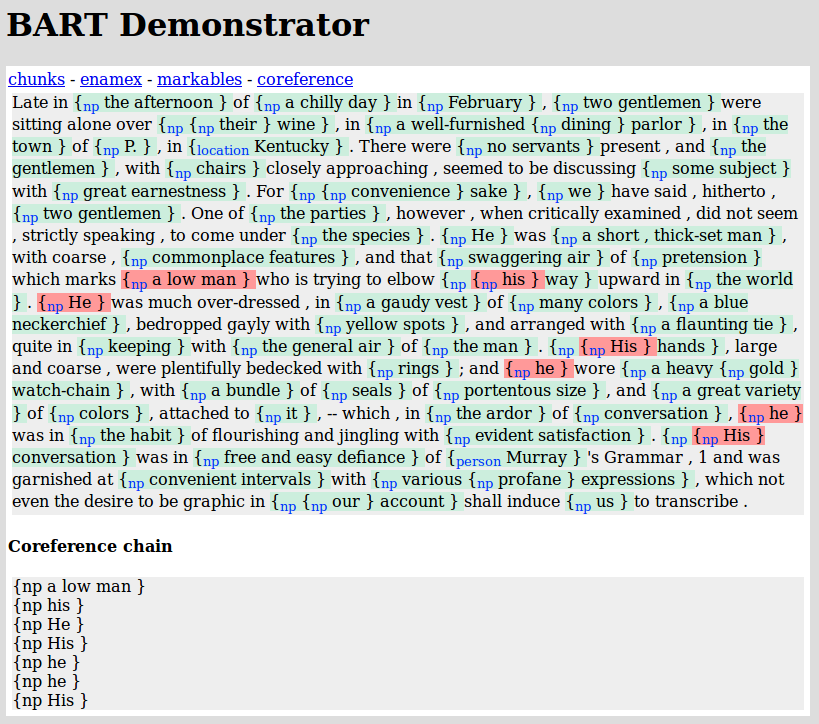
\includegraphics[width=12cm]{./img/cle/bart_webUI_output.png}
 % bart_webUI_output.png: 819x724 pixel, 72dpi, 28.89x25.54 cm, bb=0 0 819 724
\caption{BART 2.0: Output für WebInterface der Blackbox Version}
\label{bart_webUI_output}
\end{center}
\end{figure}

\subsubsection{Probleme}

\noindent
Neben der Blackbox-Version bietet BART noch eine Terminalapplikation, 
die zum Trainieren neuer Modelle genutzt werden kann.
Hierfür stehen verschiedene interne Konfigurationsdateien zur Verfügung,
die sich jedoch auf die Weiterverarbeitung beziehen und nicht den erwarteten
Input modifizieren.

Da im Projekt die Verarbeitung von Output des Stanford Parsers gewünscht war,
und wir daher auch innerhalb unserer Gruppe von der Verwendung des MMAX-Formats 
Abstand genommen haben, wurde von der Konvertierung in dieses Format abgesehen.
Eine erste Analyse der Koreferenzketten, die die WebServer-Version von BART ausgab,
unterstützte diese Entscheidung ebenfalls.




%###########################################################################

\subsection{DCoref}

% !TEX encoding = UTF-8

\subsubsection{Steckbrief}

Das Werkzeug \emph{DCoref} ist ein deterministisches Modul zur Koreferenzresolution und ist Teil der \emph{Stanford CoreNLP}. Für die Verwendung dieses Moduls ist vorausgesetzt, dass andere Module vorher auf die Eingabedaten angewendet worden sind \autocite[]{chris_stanford_dcoref}. Die Module für Wortart- und Lemmabestimmung sowie Named Entitiy Recognition und für einen Parser müssen als sogenannte Annotatoren beim Verwenden der \emph{Stanford CoreNLP} wie in Listing \ref{dcoref:required_annotators} angebeben werden.

\begin{lstlisting}[label=dcoref:required_annotators, language=Java, caption=Angabe vorausgesetzter Annotatoren in Java]
//	configure properties for pipeline of the Stanford CoreNLP
Properties properties = new Properties();
properties.setProperty("annotators", 
		"pos, lemma, ner, parse, dcoref");
//	[...] set more properties and instantiate pipeline
StanfordCoreNLP pipeline = new StanfordCoreNLP(properties);
\end{lstlisting}

\noindent Außerdem ist \emph{DCoref} grundsätzlich ein zweistufiges Modul, das mit mehreren sogenannten Sieben arbeitet. Die erste Stufe legt großen Wert auf Recall und dient der Identifizierung von vorhandenen \emph{mentions} (\hyphenquote{UKenglish}{A mention is an observed textual reference to a latent real-world entity. Mentions are associated with nodes in a parse tree and are typically realized as NPs.} \autocite[S. 385 f.]{chris_haghighi}). Die zweite Stufe siebt das Ergebnis der ersten Stufe mit mehreren Sieben aus, wobei die Siebe absteigend gemäß ihrer Precision-Werte nacheinander angewendet werden \autocite[S. 28 f.]{chris_leeetal}. 

Es gibt noch eine weitere optionale Stufe, die das Endergebnis der zweiten Stufe noch weiterverarbeitet. Dabei werden Koreferenzketten mit nur einem Element entfernt und auch \emph{mentions} entfernt, die als appositive oder copulative Textelemente auftauchen \autocite[29]{chris_leeetal}. Dieses Stufe ist optional, weil fälschlicherweise aufgeführte \emph{mentions} die Score-Werte für \emph{DCoref} nicht so sehr negativ beeinflussen wie gänzlich fehlende relevante \emph{mentions} \autocite[32]{chris_leeetal}.


\subsubsection{Probleme}

Bei der Verwendung von \emph{DCoref} sind vor allem fehlende Informationen aufgefallen. Obwohl die Dokumentation auf der Homepage des Moduls \autocite[]{chris_stanford_dcoref} zunächst sehr ausführlich erscheint, verweist sie auf Download-Links, die auf Archive verweisen, in denen Dateien fehlen, wie z.B. ein Perl-Skript, das für den CoNLL-Scorer benötigt wird ist nicht vorhanden. Dieses Skript konnte man jedoch nach einer kurzen Suche leicht finden. Obwohl angegeben ist, dass man den Pfad zu diesem Skript als Option angeben kann, scheint diese Option ignoriert zu werden und ein im Code fest vorgegebener Pfad wird trotzdem verwendet. Außerdem wird nicht angegeben, dass man neben einer Standardinstallation von Perl ein bestimmtes Paket (\emph{Algorithm-Munkres}) nachinstallieren muss, da sonst das Skript nicht ausführbar ist. Versucht man, dieses Skript trotzdem über die \emph{Stanford CoreNLP} auszuführen, erfährt man nichts von dieser speziellen Fehlerursache.

Neben der Reproduktion der Score-Werte, die für die \emph{CoNLL Shared Task 2011} bestimmt wurden, sind noch andere Optionen für den in das Modul \emph{DCoref} integrierten Scorer aufgelistet, z.B. die Verwendung des Scorers für Daten im MUC6- oder ACE2004-Format. Jedoch musste der Versuch, diesen Scorer für das MUC6-Format beim Vergleichen der Ansätze zur Koreferenzresolution zu verwenden, aus Zeitgründen ergebnislos aufgegeben werden, da die Verwendung auch nach mehreren Versuchen nicht so funktioniert hat, wie die Dokumentation es angedeutet hat. 


%###########################################################################

\subsection{Reconcile}

\subsubsection{Steckbrief}

Reconcile ist eine Art Baukasten für Koreferenzresolution. Reconcile soll es möglich machen, verschiedene Ansätze und Komponenten der Koreferenzresolution zu kombinieren und zu testen. Die Verarbeitung ist in fünf Schritte eingeteilt, welche modular und einfach anpassbar gestaltet sein sollen: Vorverarbeitung, Merkmalserzeugung, Klassifikation, Clustering und Scoring. Zur Vorverarbeitung zählen Schritte wie z.B. Zerteilung in Paragraphe, Sätze und Tokenizierung, POS-Tagging, Parsing und Named Entity Recognition. Ein Merkmal, innerhalb der Merkmalserzeugung, ist ein Substantivpaar, welches sich eine gemeinsame Eigenschaft teilt. Zwei Substantive, die im Numerus gleich sind, wären z.B. ein Merkmal. Bei der Klassifikation werden dann zwei Substantive anhand dieser Merkmale verglichen. Das Ergebnis ist ein Wert, der ausdrücken soll, wie wahrscheinlich es ist, dass beide Substantive koreferent sind. Über diese Werte wird ein Clusteringalgorithmus angewandt, um Ketten innerhalb der Koreferenzen festzustellen. Abschließend soll man mit einer implementierten Scoringfunktion das Ergebnis mit einem Goldstandart vergleichen können \autocite{reconcile2}.

Die Standartkonfiguration nutzt größtenteils \emph{Stanford OpenNLP} Werkzeuge für die Vorverarbeitung. Die hier verwendete Konfiguration ist identisch mit \autocite{reconcile}. Die Entwickler von Reconcile behaupten, es sei auf dem neusten Stand der Technik (\emph{state-of-the-art}).

\subsubsection{Probleme}
Das Hauptproblem ist eindeutig die mangelnde Dokumentation. Die Möglichkeiten zur Konfiguration und zum Testen von verschiedenen Modulen kann leider nicht problemlos ausgeschöpft werden. Da Reconcile quelloffen ist, ist es möglich sich durch den Quellcode zu arbeiten, um eine ausreichende Konfigurationsmöglichkeit zu finden - dies wird allerdings noch zusätzlich durch mangelhafte Kommentierung erschwert. Die Kommandozeilenargumente sehen es vor, eine externe Konfiguration vorzuschlagen. Es stellte sich aber heraus, dass es sich hierbei nur um einen Platzhalter handelt.

Viele der Vorvararbeitungsschritte sind dementsprechend auch nicht ersichtlich. Die Anmeldung auf der Mailingliste der Reconcile-Website schlug fehl: Es erfolgte eine Ablehnung, weil diese seltsamerweise nur für interne Entwickler gedacht ist. Es sei noch einmal hervorgehoben, dass nahezu alle genannten Vorteile von Reconcile unter der fehlenden Dokumentation leiden.


%###########################################################################
%%%%%%%%%%%%%%%%%%%%%%%%%%%%%%%%%%%%%%%%%%%%%%%%%%%%%%%%
%###########################################################################

\newpage

\section{Verlauf der Gruppenarbeit}\label{Verlauf der Gruppenarbeit} %TODO


%###########################################################################

\subsection{Vergleich}%TODO


%~~~

\subsubsection{Ausgangssituation}\label{Ausgangssituation}

Wie bereits erwähnt, wurde \emph{BART 2.0} für den Vergleich der Ansätze zur Koreferenzresolution 
als Kandidat verworfen. Übrig geblieben sind also \emph{DCoref} und \emph{Reconcile}. 
Das Ziel des Vergleichs war es, mit einem MUC-Scorer \autocite{Bagga98} anhand der Werte Precision, Recall und F-Score 
den besseren der verbleibenden zwei Kandidaten zu finden. 
Um einen Goldstandard für den Vergleich der beiden Ansätze zu erhalten, 
wurde die erste Hälfte des ersten Kapitels aus \emph{Uncle Tom's Cabin} \autocite[]{chris_uncle} 
als Testdatensatz für eine manuelle Annotierung mit Unterstützung 
des dafür vorgesehenen Softwarewerkzeugs \emph{MMAX} \autocite*[]{chris_mmax} 
verwendet \autocite[]{chris_mmax_coll}.
Diese manuelle Annotierung sollte durch zwei Gruppenmitglieder durchgeführt und dann verglichen und 
verbessert werden, bevor der daraus resultierende Goldstandard für die Bewertung 
der beiden Ansätze verwendet wurde.


%~~~

\subsubsection{Probleme mit MMAX}%TODO

Die Verwendung von \emph{MMAX} hat bereits von Anfang an zu Problemen geführt. 
Trotz der vorhandenen Dokumentation war es schwierig, \emph{MMAX} zu verwenden. 
Beide Annotatoren hatten zunächst den Eindruck, das Werkzeug nicht richtig zu verwenden. 
Ein Beispiel dafür zeigt Abbildung \ref{mmax:anzeige}.

\begin{figure}[ht]
\begin{center}
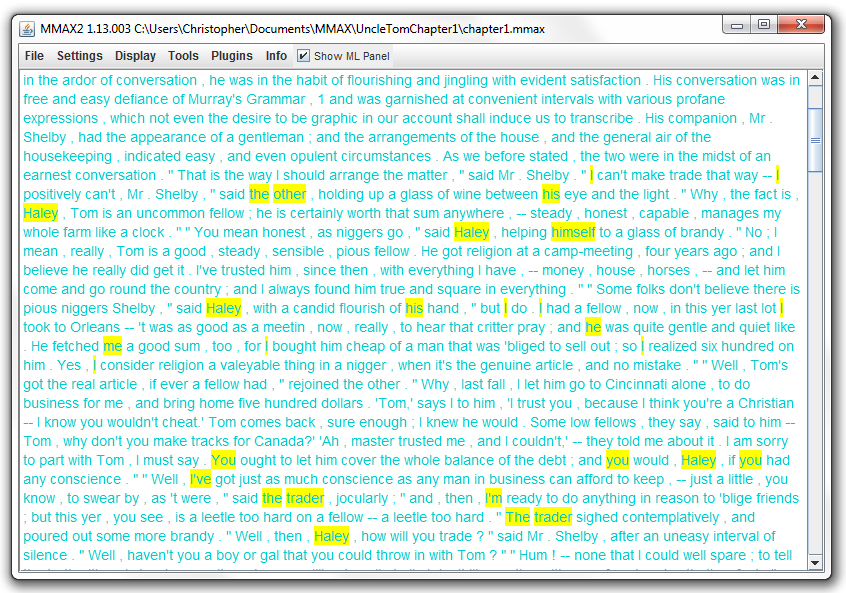
\includegraphics[width=15cm]{./img/cmich/cm_mmax.jpg}
 % bart_webUI_output.png: 819x724 pixel, 72dpi, 28.89x25.54 cm, bb=0 0 819 724
\caption{MMAX - Beispiel der Anzeige}
\label{mmax:anzeige}
\end{center}
\end{figure}

Darin ist zu sehen, wie mithilfe von \emph{MMAX} versucht wurde, eine Koreferenzkette 
für den Protagonisten \emph{Haley} in \emph{Uncle Tom's Cabin} \autocite[]{chris_uncle} zu erstellen. 
Die Hervorhebung der Kette in gelber Farbe kann über ein mit einem Rechtsklick erreichbares Kontextmenü 
aktiviert werden, allerdings findet diese Hervorhebung nur in dem im aktuellen Fensterausschnitt 
sichtbaren Teil des Textes statt. 
Die türkise Farbe war ursprünglich als Markierungsfarbe für die Kette eines bestimmten Protagonisten gedacht. 
Dieses Vorhaben hat jedoch nicht funktioniert, da jedes einzelne Wort im Text mit türkiser Farbe markiert wurde. 
Bei der Erstellung des \emph{MMAX}-Projekts für die Annotierung konnte man 
verschiedenen Annotierungsebenen unterschiedliche Farben zuordnen, 
jedoch war es nicht ohne Weiteres möglich, diese Farben sinnvoll einzusetzen, 
wie das Beispiel in der Abbildung zeigt. 
Außerdem haben mit der Zeit länger werdende Ketten vermutlich ab einer gewissen Länge Speicherprobleme verursacht 
und zu korrupten Daten geführt, die wiederholte Abstürze für \emph{MMAX} zur Folge hatten. 

Insgesamt haben diese Probleme dazu geführt, dass es nicht sinnvoll erschien, 
mehr Zeit in die Suche nach Fehlern und Alternativen bei der Konfiguration 
eines \emph{MMAX}-Projektes zu investieren. 
Das vorläufige Ziel des Vergleichs der mit \emph{MMAX} erstellten Ketten wurde folglich 
als praktisch unmöglich eingeschätzt. 
Aus diesem Grund hat sich die Frage ergeben, wie das Ziel, einen Goldstandard zu erhalten, 
auf einem anderen Weg zu erreichen ist.


%~~~

\subsubsection{Alternative Lösung}%TODO

\textbf{TODO: Standardweg: CoNLL}

Als alternativen Lösungsweg hin zu einem Vergleich der Precision-, Recall- und F-Score-Werte für \emph{DCoref} 
und \emph{Reconcile} hat sich dann die \emph{Reconcile}-Ausgabe für die Testdaten angeboten. 
Diese Ausgabe wurde manuell von zwei Annotatoren korrigiert, um einen Goldstandard zu erhalten. 
Dabei wurde das \emph{Reconcile}-Ausgabeformat beibehalten. 
Dann wurde die \emph{DCoref}-Ausgabe für die Testdaten ebenfalls in das \emph{Reconcile}-Ausgabeformat überführt, 
wie es in Listings  \ref{output:vergleich:decoref} und \ref{output:vergleich:reconcile} zu sehen ist. 
Dafür mussten lediglich die Informationen innerhalb des <coreferences>-Knotens im Reintext der Testdaten 
entsprechend als <NP>-Tags an den richtigen Stellen eingefügt werden.

\begin{lstlisting}[label=output:vergleich:decoref, name=vergleich_decoref.xml, language=xml, caption=Ausschnitt der \emph{DCoref}-Ausgabe für die Testdaten]
<?xml version="1.0" encoding="UTF-8" standalone="no"?>
<chapter id="1" title="In Which [...] Humanity">
  <sentences/>
  <coreferences>
    ...
    <coreference id="2">
      <mention representative="true">
        <sentence>1</sentence>
        <start>34</start>
        <end>35</end>
        <head>34</head>
        <text>Kentucky</text>
      </mention>
      ...
    </coreference>
    ...
  </coreferences>
</chapter>
\end{lstlisting}

\begin{lstlisting}[label=output:vergleich:reconcile, name=vergleich_reconcile.xml, language=xml, caption=Ausschnitt aus Listing \ref{output:vergleich:reconcile} im \emph{Reconcile}-Ausgabeformat]
... in <NP NO="8" CorefID="8">Kentucky</NP>. There were ...
\end{lstlisting}

\noindent 
Für die Auswertung hat ein MUC-Scorer sowohl die nicht nachbearbeitete \emph{Reconcile}-Ausgabe als auch 
die umformatierte \emph{DCoref}-Ausgabe mit dem manuell erstellten Goldstandard verglichen. 
Die Ergebnisse dieses Auswertung sind in Tabelle \ref{score:ergebnis} zu finden.

\begin{savenotes}
	\begin{table}[ht]
		\centering
  		\begin{tabular}{ l || c | c | c ||  r }
						& Reconcile 	& DCoref 	& DCoref (PP\footnote[1]{PP steht hier für das Post-Processing, das in der optionalen dritten Stufe von \emph{DCoref} stattfindet.}) 	& \\ \hline \hline
    			Precision 	& 0.99673 	& 0.74510	& 0.74837		& \\ \hline
    			Recall     	& 0.97917 	& 0.35775 	& 0.33861 		& \\ \hline
    			FScore    	& 0.98787  	& 0.48340 	& 0.46625 		& \\ \hline
  		\end{tabular}
  		\caption{Auswertung der Ansätze mit einem MUC-Scorer}
  		\label{score:ergebnis}
	\end{table}
\end{savenotes}

Offensichtlich schneidet \emph{Reconcile} viel besser ab als \emph{DCoref}. 
Dieses Ergebnis liegt wahrscheinlich auch daran, dass die \emph{Reconcile}-Ausgabe als 
Ausgangspunkt für die Annotierung verwendet wurde, da auf diese Weise der Goldstandard und 
die \emph{Reconcile}-Ausgabe nicht unabhängig voneinander entstanden sind und deshalb sehr ähnlich sind. 
Außerdem zeigt die Auswertung auch, dass die optionale dritte Stufe, 
die bei \emph{DCoref} für die Nachverarbeitung zuständig ist, 
durch das Entfernen von relevanten \emph{mentions} die Scores negativ beeinflusst, 
wie es von den Autoren auch beschrieben wurde \autocite[29, 32]{chris_leeetal}.

Da der hier vorgestellte Vergleich nicht optimal abgelaufen ist, wurde die Entscheidung getroffen, 
sowohl mit \emph{DCoref} als auch mit \emph{Reconcile} Koreferenzinformationen zu erschließen 
und die jeweilige Ausgabe wie von der dritten Gruppe gewünscht zu formatieren. 
Dabei wurden die beiden Ansätze allerdings nicht in ein einzelnes System integriert. 
Die Ausgabedaten wurden mithilfe von separaten Programmen erstellt und entsprechend umformatiert.


%###########################################################################

\subsection{Formatierung}\label{Verlauf:Formatierung}%TODO


%~~~

\subsubsection{DCoref}%TODO


Nach Absprache fügt die erste Gruppe der Projektarbeit bereits Koreferenzinformationen hinzu, da sie die \emph{Stanford CoreNLP} ebenfalls verwendet und bereits für jedes der drei für dieses Projekt ausgewählten Bücher laufen lässt. Trotzdem bietet das Java-Programm, das für das Hinzufügen von Koreferenzinformationen mithilfe von \emph{DCoref} zuständig ist, die Möglichkeit, die \emph{Stanford CoreNLP} mit diesem Modul laufen zu lassen. Allerdings ist dieses Programm aufgrund der Absprache mit der ersten Gruppe standardmäßig so eingestellt, dass nur noch die Umformatierung in das von der dritten Gruppe gewünschte Format ausgeführt wird und anschließend die Erstellung der kapitelübergreifenden Koreferenzketten ausgeführt wird (s. Abschnitt \ref{Indizierung}).

Listing \ref{input:decoref:plaintext} zeigt, dass Reintext als Eingabe erwartet wird, falls \emph{DCoref} noch Koreferenzinformationen hinzufügen muss, bevor die Ausgabe umformattiert wird. Der dafür gewählte Beispieltext stellt den eindeutigen Endpunkt der ersten Hälfte des ersten Kapitels im Buch \emph{Uncle Tom's Cabin} \autocite[]{chris_uncle} dar, der für die Testdaten vereinbart wurde (s. Abschnitt \ref{Ausgangssituation}).

\begin{lstlisting}[label=input:decoref:plaintext, name=decoref_in_plain.xml, language=xml, caption={Reintext, Eingabe für \emph{DCoref}}]
...
And the trader leaned back in his chair, and folded his arm, with an air of virtuous decision, apparently considering himself a second Wilberforce. 
\end{lstlisting}

\noindent Die Ausgabe \emph{DCoref} ist in Listing \ref{output:decoref:unformatiert} zu sehen. Bei diesem Format sind zwei Dinge negativ aufgefallen. Einerseits kommt der <coreference>-Tag auf zwei verschiedene Arten vor: Er wird nicht nur für den Sammelknoten verwendet, der die eigentlichen XML-Knoten für die einzelnen Ketten enthält, sondern auch für die Knoten der Koreferenzketten selbst. Deshalb hat die dritte Gruppe um eine Umbenennung der Sammelknoten-Tags von <coreference> in <coreferences> gebeten. Für die Knoten der Koreferenzketten wurde außerdem eine eindeutige Nummerierung in Form eines \emph{id}-Attributs gebeten. 

\begin{lstlisting}[label=output:decoref:unformatiert, name=decoref_out.xml, language=xml, caption={XML, Unformatierte Ausgabe von \emph{DCoref}}]
<?xml version="1.0" encoding="UTF-8"?>
<?xml-stylesheet href="CoreNLP-to-HTML.xsl" type="text/xsl"?>
<root>
  <document>
    <sentences/>
    <coreference>
      ...
      <coreference>
        <mention representative="true"/>
        ...
      </coreference>
      ...
    </coreference>
  </document>
</root>
\end{lstlisting}

\noindent Durch eine Umformatierung werden die von der dritten Gruppe beschriebenen Mängel behoben. Dadurch wird das ursprüngliche Ausgabeformat von \emph{DCoref} in das in Listing \ref{output:decoref:formatiert} gezeigte endgültige Format gebracht. Dieses Format ist ebenfalls gruppenintern für die Schnittstelle zum Programm für die Erstellung der kapitelübergreifenden Koreferenzketten festgelegt worden.   

\begin{lstlisting}[label=output:decoref:formatiert, name=decoref_out_formatted.xml, language=xml, caption={XML, Formatierte Ausgabe von \emph{DCoref}}]
<?xml version="1.0" encoding="UTF-8" standalone="no"?>
<chapter id="1" title="In Which [...] Humanity">
  <sentences/>
  <coreferences>
    ...
    <coreference id="1">
      <mention representative="true">
      ...
    </coreference>
    ...
  </coreferences>
</chapter>
\end{lstlisting}

\noindent Das Programm für \emph{DCoref} bietet auch die Möglichkeit, die optionale dritte Stufe des Moduls auszuführen. Die Dateien, die bei der Auswahl dieser Option erstellt werden, werden entsprechend gekennzeichnet bzw. in separaten Ordnern abgelegt, um sie von eventuell bereits vorhandenen anderen Dateien zu unterscheiden. Diese Unterscheidung betrifft die Ausgabedateien der ersten Gruppe für jedes einzelne Kapitel sowie die durch den Aufruf des Programms für die Erstellung kapitelübergreifender Ketten erstellte Indexdatei. Weitere Details zu der verwendeten Ordnerstruktur und zu dieser Unterscheidung befinden sich in den im Rahmen des Projektes verwendeten öffentlichen \emph{GitHub}-Repositories (s. Abschnitt \ref{Repositories}).


%~~~

\subsubsection{Reconcile}

Das Reconcileausgabeformat ermöglicht es mit einem leicht modifizierten XML-Parser die Koreferenzierungen zu extrahieren. Diese teilweise rekursiven Strukturen besitzen zwei Attribute: Eine eindeutige Identifizierungsnummer und einen Verweis auf das Kopfelement in Form von deren Identifizierungsnummer. Handelt es sich bei dem Element um einen Kopf, sind beide Zahlen identisch. Die gewünschte Darstellungsform der dritten Gruppe lässt sich ausdrücken als quasi transitive Hülle für die Koreferenzköpfe. Mit dieser Betrachtung konnten die Ketten aus der Ausgabedatei extrahiert und zusammengeführt werden.

Da in der benutzten Reconcilekonfiguration bereits die \emph{OpenNLP} Werkzeuge verwendet wurden, konnte man davon ausgehen, dass sowohl die Paragraphen- und Satzeinteilung, wie auch die Tokenisierung, identisch mit der Ausgabe der ersten Gruppe ist. Das Problem war allerdings, dass viele der benötigten Informationen nicht mehr in der Ausgabe von Reconcile enthalten waren. Es gab keine Informationen über die Nummer des Satzes oder der Token oder den Kopf der \emph{mention}. Da es nicht ersichtlich war wie Reconcile die Ausgabe gestaltet, mussten diese Informationen für die Umwandlung noch nachträglich berechnet werden.

Die Umformung läuft in folgenden Schritten ab. Zuerst werden die Sätze der Reconcileausgabe nummeriert. Für jeden Satz werden mittels eines XML-Parsers die ausgezeichneten Koreferenzen extrahiert und mit der Information über die Satznummer ergänzt. Für jeden Satz im Orginaltext werden die Token nummeriert. Diese Information wird für die Ketten ergänzt. Nun ist es möglich, die Tokennummer des Phrasenkopfes berechnen zu lassen. Von jeder Koreferenz wird danach deren transitive Hülle gebildet. Diese Datenstruktur besitzt jetzt alle nötigen Informationen für die Schnittstelle zur dritten Gruppe. Die Datenstruktur wird abschließend in XML umgewandelt.


%###########################################################################

\subsection{Indizierung}\label{Indizierung}

% !TEX encoding = UTF-8
\subsubsection{Coref.java}
mainklasse
  
  I/O Parser
  
  Usage msg
  
  call InputAnalyzer for each input.xml
  
  create map for coreferences with Coreference objects
  
  pass to OutputWriter
  
  call OutputWriter

\subsubsection{Coreference.java}
class def of Coreference objects
  
  attr.s text chapId corefId

\subsubsection{InputAnalyzer.java}
extract coref information
  
  create Map of Coreference object
  
    analyze input.xmls with jdom
    
    extract chapterID, corefID, representative mention text-element
    
    create Coreference object 
    
      ->pass to Map of Coreference object

\subsubsection{OutputWriter.java}
multimap with representative text as key and Coreference objs

  create ArrayList if key not already existent

  add coreference for key to ArrayList in multiMap for key

  create output element
  
    write basic elements
    
    create sub elements for each coref in outputdoc
  
Write the complete result document to output XML file


%###########################################################################
%%%%%%%%%%%%%%%%%%%%%%%%%%%%%%%%%%%%%%%%%%%%%%%%%%%%%%%%
%###########################################################################

\newpage

\section{Zusammenfassung}%TODO


%###########################################################################

\subsection{Aufgabenverteilung}%TODO

Bei der Bestimmung der Kandidaten für die Auswahl eines geeigneten Ansatzes für die Koreferenzresolution 
hat jedes Gruppenmitglied einen Ansatz übernommen. 
Clemens Ahrens hat sich mit \emph{BART 2.0} beschäftigt, André Beyer mit \emph{Reconcile} und 
Christopher Michels mit \emph{DCoref}.

Während Clemens Ahrens ein Programm für die Erstellung kapitelübergreifender Koreferenzketten entwickelt hat 
und nachdem \emph{BART 2.0} als Kandidat verworfen wurde, 
haben sich André Beyer und Christopher Michels mit dem Vergleich von \emph{DCoref} 
und \emph{Reconcile} beschäftigt. 
Nach vergeblichen Versuchen, \emph{MMAX} und in die betrachteten Softwarewerkzeuge integrierten Scorer 
für diese Aufgabe zu verwenden, wurde ein Goldstandard im \emph{Reconcile}-Ausgabeformat erstellt. 
Dann hat André Beyer einen MUC-Scorer für das gleiche Ausgabeformat entwickelt. 
Um \emph{DCoref} ebenfalls mit diesem MUC-Scorer bewerten zu können, 
hat Christopher Michels die Ausgabe von \emph{DCoref} für die Testdaten entsprechend umformatiert.

Außerdem hat André Beyer ein Programm zur Umformatierung der Ausgabe von \emph{Reconcile} für das 
von der dritten Gruppe geforderte Ausgabeformat geschrieben. 
Analog hat Christopher Michels die Ausgabe von \emph{DCoref} für die Schnittstelle der dritten Gruppe umformatiert. 
Clemens Ahrens hat mithilfe von ersten funktionierenden Programmversionen unserer Gruppe vorläufige Testdaten 
für das Buch \emph{Uncle Tom's Cabin} \autocite[]{chris_uncle} an die dritte Gruppe weitergegeben, 
damit diese neben selbsterstellten Daten weiteres Testmaterial zur Verfügung hatte.

%###########################################################################

\subsection{Kommentar EVENTUELL?}\label{Kommentar}%TODO

TODO: Sowas wie eine kurze abschließende Bewertung vielleicht? 
Mir (Chris) ist nur nichts Gutes eingefallen und ich muss noch für eine Klausur lernen. 
Wenn ich noch unbedingt was selbst ändern soll, sagt mir bitte bescheid. 
Wenn niemand sonst will, lassen wir es weg ...
Clemens: ich denke nicht, dass wir hier noch was brauchen.


%###########################################################################

\subsection{Repositories}\label{Repositories}

Die folgenden öffentlichen Repositories wurden auf \emph{GitHub} \autocite[]{chris_github} im Rahmen 
der Gruppenarbeit erstellt und verwendet. 
Dort sind weitere Details der erstellten Programme sowie Informationen zu deren Verwendung einsehbar.

\begin{itemize}
  \item Umwandler von \emph{Reconcile} zur Schnittstelle der dritten Gruppe:\par \url{https://github.com/beyeran/transform-reconcile}\vspace{0.3cm}
  \item MUC Scorer für die \emph{Reconcile}-Dateien:\par \url{https://github.com/beyeran/score-coref}\vspace{0.3cm}
  \item Umwandlung von \emph{DCoref} zur Schnittstelle der dritten Gruppe:\par \url{https://github.com/cmich/dh-projekt-gruppe2-dcoref}\vspace{0.3cm}
  \item \emph{DCoref} für die Eingabedaten:\par \url{https://github.com/Rostu/dh-Projekt-Gruppe1}\vspace{0.3cm}
  \item Erstellung der Indexdatei für kapitelübergreifende Koreferenzketten: \par \url{https://github.com/ClemensAhrens/BuildIndex}\vspace{0.3cm}
\end{itemize}


%###########################################################################
%%%%%%%%%%%%%%%%%%%%%%%%%%%%%%%%%%%%%%%%%%%%%%%%%%%%%%%%
%###########################################################################

\newpage

% \printshorthands[title=Abkürzungsverzeichnis]
\printbibliography[title=Literaturverzeichnis, heading=bibintoc]


\end{document}
